\documentclass[11pt,german]{scrartcl}

% See geometry.pdf to learn the layout options.
\usepackage{geometry}
\geometry{a4paper}

% To begin paragraphs with an empty line
\usepackage[parfill]{parskip}

% Use utf-8 encoding for foreign characters
\usepackage[utf8]{inputenc}

% Setup for fullpage use
\usepackage{fullpage}

% use multicol package
\usepackage{multicol}

% use multirow package
\usepackage{multirow}

% Running Headers and footers
\usepackage{fancyhdr}
\pagestyle{fancyplain}

\usepackage{url}
\usepackage{makeidx}
\usepackage[colorlinks=true, linkcolor=blue, urlcolor=blue]{hyperref}

% Surround parts of graphics with box
\usepackage{boxedminipage}

% Package for including code in the document
\usepackage{listings}
\usepackage{color}
\usepackage{moreverb}

% match packages
\usepackage{amsmath}

% Alternative monospaced font
\usepackage[T1]{fontenc}
\usepackage[scaled]{beramono}		% Debian: texlive-fonts-extra

%listings config
\definecolor{light-gray}{gray}{0.95}

\lstset{
	language={[x86masm]Assembler},                  % choose the language of the code
	                                % size of fonts used for the code
	basicstyle=\ttfamily\footnotesize,
	%numbers=left,                   % where to put the line-numbers
	numberstyle=\footnotesize,      % size of fonts for used line-numbers
	stepnumber=1,                   % step between line-numbers
	numbersep=10pt,                  % how far the line-numbers are from the code
	backgroundcolor=\color{light-gray},  % choose background color. You must add \usepackage{color}
	showspaces=false,               % show spaces adding particular underscores
	showstringspaces=false,         % underline spaces within strings
	showtabs=false,                 % show tabs within strings adding particular underscores
	frame=single,                   % adds a frame around the code
	tabsize=4,                      % sets default tabsize to 2 spaces
	captionpos=b,                   % sets the caption-position to bottom
	breaklines=true,                % sets automatic line breaking
	breakatwhitespace=false,        % sets if automatic breaks should only happen at whitespace
	escapeinside={\%*}{*)},         % if you want to add a comment within your code
  frameround=tttt,
  extendedchars=true,
  literate=%
    {Ö}{{\"O}}1
    {Ä}{{\"A}}1
    {Ü}{{\"U}}1
    {ß}{{\ss}}2
    {ü}{{\"u}}1
    {ä}{{\"a}}1
    {ö}{{\"o}}1
    {°}{{}}0
}

\makeindex

\title{Intel x86 Assembler\\\small{Proseminar Programmiersprachen}}
\author{Sebastian Raitza, Nico von Geyso}


\begin{document}

\maketitle

%\begin{abstract}
Abstract-text....
\end{abstract}


\tableofcontents

\section{Einführung}
Während vor einigen Jahren das Wissen über die Assembler-Programmierung noch unabdingbar war, ist es heute ein leichtes Unterfangen gar komplexe Probleme in einer Hochsprache zu lösen ohne jemals hardwarenah programmiert zu haben.
Der Artikel versucht die geschichtliche Entwicklung der x86-Architektur und seine Besonderheiten knapp darzustellen.
Neben Syntax und Semantik des x86 Assemblers wird auch auf das immer mehr populär werdende Thema des \textit{Reverse Engineering} eingegangen.


\section{Geschichte}

\begin{frame}{Geschichte}
	\textbf{Intel Corporation in den 70er Jahren}
	\begin{itemize}
		\item eine von vielen Chip-Herstellern
		\item starke Konkurrenz mit Zilog Incorporation und seinem Z80 Mikrocontroller
		\item vorherrschende Word-Größe war 8 Bit
		\item Verzögerung der neuen Prozessorgeneration von Intel (32 Bit)
	\end{itemize}
\end{frame}

\begin{frame}{Geschichte}
	\textbf{Intels Antwort auf den Z80}
	\begin{itemize}
		\item 8086 16 Bit Mikroprozessor
	 	\item entwickelt von einem Team um Stephen Morse 
	\end{itemize}

	$\rightarrow$ bedingt ein Erfolg
\end{frame}

\begin{frame}{Geschichte}
	\textbf{IBMs \textit{Personal Computer}	1981}
	\begin{itemize}
		\item Ziel: preisgünstiger Computer
		\item basierend auf Intels 8088-Mikroprozessor
	\end{itemize}

	$\rightarrow$ Kassenschlager und Grundstein für den Siegeszug der x86-Architektur 
\end{frame}

\begin{frame}{Geschichte}
	\begin{quote}
	Any bright engineer could have designed the processor. It would probably have had a radically different instruction set, but all PCs today would be based on that architecture instead.
	\end{quote}

	\textit{Stephen Morse}
\end{frame}

\begin{frame}{Geschichte}
	\begin{quote}
	If IBM had chosen the Motorola 68000 for the IBM PC (as some wanted), we would have had the WinOla duopoly rather than the Wintel duopoly
	\end{quote}
	\textit{Bradley (IBM)}
\end{frame}


\section{Syntax}

In der Welt des x86-Assmblers gibt es zwei große Syntaxfamilien: die Intel und
die AT\&T-Syntax. Während Erstere in einer Vielzahl von Assemblern (NASM, TASM,
MASM, YASM, usw.) und Disassemblern (IDA Pro, OllyDbg) zur Standardsyntax zählt
und Intel die x86-Platform damit dokumentiert, ist Letztere dennoch nicht
gänzlich irrelevant. In der UNIX und Linux-Welt wurde lange Zeit nur AT\&T's
Syntaxstil von den ausgelieferten Assemblern \texttt{as} bzw. \texttt{gas}
unterstütlich. Insbesondere durch die Verbreitung der GNU Compiler Collection
hat sich dieser Stil bis heute gehalten, obwohl der GNU Assembler mittlerweile
auch die Intel-Syntax beherscht.

Überhaupt sind die Unterschiede breider Stile gleichmächtig und lassen sich
trotz erheblicher optischer Unterschiede problemlos ineinander konvertieren
(z.B. mit Intel2GAS \cite{i2g}). Für die Folgenden Beispiele wird die
Intel-Syntax als die kanonische Referenz betrachtet und jeweils der
äquivilenten AT\&T-Syntax gegenübergestellt.

% [i2g] http://www.niksula.hut.fi/~mtiihone/intel2gas/

\subsection{Arebitsweise des Assemblers}

Programmiert man mit einem Assembler, wie z.B. NASM, so beschreibt man Zeile
für Zeile je eine Prozessorinstruktionen über ihr Symbol, einem sogenannten
Mnemonic's gefolgt von den dazugehörigen optionalen Argumenten. Die Funktionen
des Assemblers ist es nun dieses Symbolische Programm direkt in die
entsprechende Folge binären x86-Maschinencode – man spricht von Opcodes, die
üblicherweise byteweise, hexadezimal dargestellt werden.

Vereinfach gesagt bedient sich der Assembler einer großen Symboltabelle in der
für jedes Tupel von Mnemnonic und Argumenten der entsprechende Opcode vermerkt
ist. Der Programmierer könnte zwar selbst direkt in Opcodes programmieren und
bekommt aber dadurch die Erleichterung sich statt Hexadezimal-Codes nur Symbole
merken zu müssen.

\subsection{Instruktionen}

Eine Zeile in einem Assemblerprogramm hat folgende Form und ist in beiden
Syntaxstilen gleich:

\texttt{[label:] mnemonic [argument1][, argument2][, argument3]}

Label ist eine Sprungmarke und optional, ebenso wie die Argumente. Deren
erforderliche Anzahl hängt von der Instruktion ab. Maximal drei, häufiger zwei
Argumente sind üblich. Das Mnemnonic bzw. Instruktionssymbol ist eine kurze
Zeichenkette, wie zum Beispiel MOV, ADD oder PUSH, und abstrahiert gleich über
eine Klasse von Opcodes mit derselben Funktion.\cite{intelmanual} So ist zum
Beispiel die Kopieroperation für Argumente verschiedene Art (Register,
Konstanten) immer das Mnemnonic MOV obwohl sich die Opcodes unterscheiden.

Groß- und Kleinschreibung wird nicht unterschieden.

\subsection{Parameter}

Bei vielen Befehlen sind zwei Argumente üblich. Es wird dann meist von Quell-
und Zieloperanden gesprochen (source and destination parameter). Die Semantik
der Parameterreihenfolge bei Intel-Syntax entgegengesetzt zur AT\&-Syntax.

Ein Parameter kann von dreierlei Art sein: ein Register, eine Konstante oder
Speicheradresse. Die Registerbezeichnungen (z.B. EAX, EBP) sind bei Intel und
AT\&T identisch, allerdings erfodert Letztere noch ein Prozentzeichen im
Prefix. Konstanten erhalten bei AT\&T ein Dollarzeichen-Prefix. Intel-Assembler
benötigt diese Kennzeichnung nicht.

\hspace{5mm} \makebox[1.5cm]{Intel: \hfill}
\texttt{mov eax, 5}

Eine weitere Eigenart der AT\&T-Syntax ein Befehls-Suffix b, w, l, oder q, der
die Parametergröße beschreibt: Byte, Word (16 Bit), Long oder Double-Word  (32
Bit) bzw.  Quad-Word (64-Bit). Für Intels Syntax leitet der Assembler den Typ
automatisch vom Parameter ab.

\hspace{5mm} \makebox[1.5cm]{AT\&T: \hfill}
\texttt{mov \$5,\%eax}

Ein Parameter kann eine absolute Adresse enthalten oder indirekt auf den Inhalt
einer Speicherstelle zeigen. Die Speicheradresse für die Derefeerenzierung kann
aus einem Ausdruck berechnet werden.  Diese effektive Adresse wird bei Intel
aus Variblen in eckigen Klammern gebildet und kann eine Typangabe wie
\texttt{BYTE},  \texttt{WORD} und \texttt{DWORD} gefolgt von  \texttt{PTR}
(Pointer) vorangestellt bekommen.

\hspace{5mm} \makebox[1.5cm]{Intel: \hfill}
\texttt{mov eax, dword ptr [ebp+4]}

In AT\&T Syntax berechnet sich eine Adresse nach dem sogenannten \emph{base
indexed addressing}-Schema aus den Einzelkomponenten Adresse (auch
\emph{disposition}), Basis, Index, Skalierung, wie folgt: $Adresse + Basis +
Index*Skalierung$ . Ein Beispiel:

\hspace{5mm} \makebox[1.5cm]{AT\&T: \hfill}
\texttt{movl 4(\%ebp), \%eax}

Die wesentliche Syntax-Unterschiede sind in der Tabelle~\ref{tab:syntaxdiffs}
zusammengefasst.

%\clearpage

\begin{table}[h]	% place here
\begin{tabular}{lll}
\\	                          & INTEL SYNTAX                  &        AT\&T SYNTAX
\\\hline
\\	Parameter 								& \tt mnem dest, src, const  	  & \tt mnem src, dest, const
\\Adressierung  				    	&	\tt [base+index*scale+disp]   & \tt disp(base, index, scale)
\\	Register      						& \tt eax              					& \tt \%eax
\\	Konstante     						& \tt 0xFF             					& \tt \$0xFF
\\	Dereferenzieung   				& \tt [addr]           					& \tt addr(,1)
\\	Absolute Adresse 			 	  & \tt addr             					& \tt *addr
\\	{\tt byte} Instruktion    & \tt mov byte ptr     					& \tt movb
\\	{\tt word} Instruktion    & \tt mov word ptr     					& \tt movw
\\{\tt dword} Instruktion     & \tt mov dword ptr    					& \tt movl
\end{tabular}
\caption{Syntax Unterschiede} \label{tab:syntaxdiffs}
\end{table}



\subsection{Segmente} Jeder x86 Quellcode ist in verschiedene Segmente
unterteilt. Da wären zum einen die Datensegmente die mittels den
Schüsselwörtern \texttt{.data} und \texttt{.stack} definiert werden, sowie
letztendlich das Codesegment. Im letzteren steht das eigentliche Programm,
während im ersterem unter anderem Speicher alloziert und initialsiert wird.


%Register
%Adressierung
%Register
%Adressierung
\section{Architektur}
X86-Assembler umfasst eine Instruktionsmenge die ursprünglich für Intels 8086 CPU konzipiert war. Diese basiert auf einer "von Neumann"-Architektur. Hier wird, im Gegensatz zur Harvard-Architektur, für Daten und Programme der gleiche Speicher verwendet. Es existierte ein fester Registersatz von 16 Registern der sich im Laufe der Zeit immer weiter vergrößert hat. Ursprünglich hatte x86 vier general-purpose Register (AX, BX, CX und DX), vier Segmentregister zur Speicheradressierung (CS, DS, ES und SS), vier Indexregistern (SP, BP, SI, DI), sowie dem FLAG-Register und dem Instruktionszeiger-Register.

\subsection{Prozessor-Register}

Der Registersatz wurde im Laufe der Zeit mit jeder neuen Prozessorgenerationen erweitert. Wichtigster Schritt war dabei die Einführung von 32-Bit Registern mit dem 80386. Alle 16-bit Grundregister mit Ausnahme der Segmentregister wurden in ihrer Größe verdoppelt und mit dem Präfix E versehen. Mit der Einführung von 32-Bit Registern, Adressbus und Instruktionen spricht man auch von der IA-32 Plattform (\emph{Intel Architecture, 32-bit)}.

\subsubsection{Allzweckregister}

\begin{tabular}{|c|l|l|}
\hline EAX & \emph{accumulator} & AX, AH, AL \\
\hline EBX & \emph{base register} & BX, BH, BL \\
\hline ECX & \emph{counter register} & BX, CH, CL \\
\hline EDX & \emph{data register} & DX, DH, DL \\
\hline \end{tabular}

Die vier Allzweckregister, \emph{general-purpose} oder auch Rechenregister dienen als Operanden für vielerlei Instruktionen und ermöglichen eine freie Manipulation der Daten mit denen der Prozessor rechnet.

Sie besitzen seit dem 80386 eine Größe von 32-bit – in der Intel-Sprache ein DWord (\emph{double-word}, wird so bezeichnet da ein Prozessorwort ursprünglich aus 16-bit beinhalten konnte). Die alten Bezeichner {\tt AX, BX, CX} und {\tt DX} können nach wie vor verwendet werden und meinen dann die unteren 16-Bit des Registers.

Darüber hinaus war es beim 8086 möglich die Allzweckregister in zwei Teilen anzusprechen: dem \emph{High-Byte} für Bits 8-15 in {\tt AH, BH, CH} für  und {\tt DH} und dem \emph{Low-Byte} mit Bits 0-7 in {\tt AL, BL, CL} und {\tt DL}. Eine Operation auf einen dieser 8-bit Hälften geschieht ohne Seiteneffekte auf jeweils andere.

Obwohl fast alle Rechenoperationen auf alle vier Register angewendet werden können, erfüllen sie für manche Instruktionen spezielle Aufgaben. Genaue Angaben findet der Programmierer dazu zum Beispiel in Intels Referenz-Dokumentation. \cite{intelreferenz}

Ein Compiler legt über seine Aufrufkonvention oft fest ob den Registern besondere Aufgaben zukommen sollen. So wird {\tt EAX} von vielen C-Compilern immer als Register für den Rückgabewert eines Funktionsaufrufs benutzt. \cite{wp:callconv}

\subsubsection{Segmentregister und Adressierung}

\begin{tabular}{|c|l|}
\hline CS & \emph{code segment} \\
\hline DS & \emph{daten segment} \\
\hline SS & \emph{stack segment} \\
\hline ES, FS, GS & \emph {extra segment registers} \\
\hline
\end{tabular}

Die Segmentregister sind als einzige Register 16-Bit breit geblieben und lassen sich nicht in byteweise aufteilen. Das hängt mit ihrer speziellen Funktion zusammen, denn sie nehmen Anfangsadressen von Segmenten im Speicher auf. Dies ist nützlich zur Bildung von Pointern. Die Adresse des Stack-Speichers wird so zum Beispiel über das Registerpaar SS:ESP ermittelt. Vor dem 80386 Prozessor waren sie besonders relevant für die sogenannte segmentierte Adressierung im \emph{Real Mode} um die vollen 20-Bit des Adressbusses bei nur 16-Bit Registerbreite bei der Adressierung verwenden zu können.
Segmentregister können immer nur mittels eines Allzweckregisters oder spezielle Instruktionen gesetzt werden.

% lassen sich lediglich auslesen und beschreiben

\subsubsection{Zeige- und Indexregister}

Diese Register sind nützlich als Zeiger auf Datenstrukturen, Indexierung in Arrays und bei String-Manipulation und als Offset als Teil einer Adresse. Sie lassen sich mit den Segmentregistern kombinieren, um in weit entfernte Speicherbereiche zu zeigen. 

\begin{tabular}{|c|l|l|}
\hline ESI & \emph{source index} & DS:ESI, SI\\
\hline EDI & \emph{destination index} & ES:EDI, DI\\
\hline
\end{tabular}

ESI und EDI dienen als String und Speicherkopieroperationen in Arrays und lassen sich mit DS bzw. DS kombinieren.

\begin{tabular}{|c|l|}
\hline ESP & \emph{stack pointer} SS\\
\hline EBP & \emph{base pointer} SS\\
\hline
\end{tabular}

Die Zeiger für den Stack {\tt ESP} und {\tt EBP} dienen zum Aufspannen eines Stackbereich bei Funktionsaufrufen. {\tt ESP} zeigt dabei immer auf das oberste Element im Stack und wird bei {\tt push}- und {\tt pop}-Befehlen manipuliert, während {\tt EBP} auf eine anderen Adresse im Stack zeigen kann um die Basis eines Stackbereichs zu definieren. Das Stack-Segmentregister SS definiert das aktuelle Speichersegment für die Offsets in {\tt ESP} und {\tt EBP}.

\begin{tabular}{|c|l|}
\hline EIP & \emph{instruction pointer} \\
\hline
\end{tabular}

Der Instruktionszeiger ist ein spezielles Register und zeigt immer auf den aktuell nächsten Befehl in der Ausführung. Der {\tt EIP} wird ausschließlich intern durch den Prozessor verändert – der Programmieren manipuliert diesen indirekt über bedingte und unbedingte Sprungbefehle. Bei Unterfunktionsaufrufen wird der aktuelle {\tt EIP}, der  auf die nächste Instruktion hinter {\tt call} zeigt, automatisch auf den Stack gelegt und bei der Rückkehr mittels {\tt ret} an diese Adresse zurückverzweigt.

\subsubsection{Statusregister}

Das Register {\tt EFLAGS} enthält Informationen über den aktuellen Zustand des Prozessors in Form von binären Flags. Die unteren 16-Bits (ursprünglich das 8086-Register {\tt FLAGS}) haben untenstehende Bedeutung. Die 32-Bit des {\tt EFLAGS} erhält noch einige zusätzliche Flags.

{\small 15}
\begin{tabular}{|c|c|c|c|c|c|c|c|c|c|c|c|c|c|c|c|c|}
\hline & & & & O & D & I & T & S & Z & & A & & P & & C \\
\hline
\end{tabular}
{\small 0}

\emph{overflow, direction, interrupt, trap, sign, zero, auxiliary, parity}
und \emph{carry flag} 

\subsection{Adressraum}

\subsubsection{Real Mode}

16 bit Mode, seit 8086

Segmentregister (CS, DS, SS, ES) sind relevant für segmentierte Adressierung im
\emph{Real Mode} um über statt 16 Bit zur Adressierung, 20 Bit zu verfügen

$Adresse = 16 * Segment + Offset$

Dies erhöht den Adressraum von 64 KByte auf 1 MByte.


\subsubsection{Protected Mode}
Im \emph{protected mode} mit 32-Bit Adressierung werden alle 16-Bit auf 32-Bit erweitert

\texttt{SEGMENT:OFFSET} Adressierung ist ebenfalls möglich, aber weniger relevant als im
\emph{Real Mode}, da nun volle $2^{32}$-Bit (4 GByte) adressiert werden können




Arten der Adressierung:

\begin{enumerate}
\item Direktwertadressierung (Immediates)
\item Direkte Adressierung
\item Indirekte Registeradressierung
\item Indizierte Registeradressierung
\end{enumerate}


% \section{Unterprogramme}


\section{Instruktionen}

Anders als in Hochsprachen wird bei der Assemblerprogrammierung meist mit Registern gearbeitet.
Auf diese können dann Instruktionen angewendet werden. Diese sind in ihrer Anzahl limitiert.

\subsection{Daten kopieren}
%Introduction to 80x86 Assembly Language and Computer Architecture - Seite 86
Eine der am häufigsten verwendeten Operationen ist das Kopieren von Daten vom Speicher in ein Register und wieder zurück.
Darunter fällt auch das Zuweisen eines konstanten Wertes eines Registers oder einer Speicherzelle.
Hierzu wird im x86-Assembler das \texttt{mov}-Mnemonic verwendet.
Es können immer nur Daten der gleichen Größe kopiert werden.
Das heißt es muss sichergestellt sein, dass die Register beziehungsweise Adressen dementsprechend gleich große Werte speichern können.
Wichtig ist, dass es sich bei einer der beiden Adressen immer um ein Register handeln muss.

Im folgendem Beispiel wird in das Register \texttt{eax} der Wert aus dem Register \texttt{ebx} kopiert:

\begin{lstlisting}
mov    eax, ebx
\end{lstlisting}

Um einer Zieladresse einen festen Wert zu zuweisen, kann statt einer \textit{Source-Adresse} auch eine Konstante stehen:

\begin{lstlisting}
mov    eax, 5
\end{lstlisting}

Im Register \textit{eax} steht nun nach erfolgreicher Abarbeitung der Instruktion der Wert 5.


\subsection{Arithmetische und logische Funktionen}
%inc,dec,add,sub,xor
%Introduction to 80x86 Assembly Language and Computer Architecture - Seite 96
Meist werden die mathematischen Basisoperationen in der Hardware mit Hilfe der ALU\footnote{Arithmetisch-logische-Einheit} berechnet.
Hierzu zählen arithmetische Funktionen, wie die Addition und Subtraktion, sowie logische Funktionen.

Mittels des \texttt{INC}-, sowie des \texttt{DEC}-Mnemonics können Register in- beziehungsweise dekrementiert werden. Um zwei Register zu addieren oder subtrahieren, wird das \texttt{ADD}- beziehungsweise das \texttt{SUB}-Mnemonic verwendet.

Da bei einigen Operationen Sonderfälle auftreten können, werden Informationen diesbezüglich in den sogenannten \textit{Flag}-Registern gespeichert.
Hier kann überprüft werden ob das Ergebnis negativ oder null ist, sowie festgestellt werden ob es einen Überlauf gab.

\paragraph{Beispiel\newline}\makebox{}

\begin{lstlisting}
mov    eax, 255  ; Register eax wird der Wert 255 zugewiesen
add    eax, 5    ; Addition: eax + 5 = 260 
\end{lstlisting}

In unserem Beispiel für 8-Bit große Register führt die Addition zu einem \textit{Overflow}.
Dies ist ein Sonderfall und dadurch wird das entsprechende \textit{O}-Flag\footnote{Overflow Flag} gesetzt.

Ein Blick auf die \textit{Flag}-Register zeigt uns genau dies:

\begin{tabular}{|c|c|c|c|c|c|c|c|c|c|c|c|c|c|c|c|c|c|}
\hline Werte & 0 & 0 & 0 & 1 & 0 & 0 & 0 & 0 & 0 & 0 & 0 & 0 & 0 & 0 & 0 & 0 \\
\hline Register & & & & O & D & I & T & S & Z & & A & & P & & C & \\
\hline
\end{tabular}

\subsection{Vergleiche}
Bei der Lösung von Problemen ist man als Programmierer oft auf Vergleiche zwischen Werten angewiesen.
Hier gibt zwei Mnemonics um Operanten zu vergleichen. Zum einen das \texttt{test}- und das \texttt{cmp}-Mnemonic.
Der Unterschied zwischen beiden ist die mathematische Umsetzung der Operation. Während beim ersteren beide Operanten logisch miteinander verundet werden, werden beim letzteren diese einfach voneinander abgezogen. 

\paragraph{Überblick}
\begin{itemize}
	\item \texttt{cmp arg1, arg2} $\leftrightarrow \text{arg1} - \text{arg2}$

	\item \texttt{test arg1, arg2} $\leftrightarrow \text{arg1} \wedge \text{arg2}$
\end{itemize}

Das Ergebnis kann nur anhand der gesetzten \textit{Flags} ausgelesen werden.
Welche \textit{Flag}-Kombinationen für das \texttt{CMP}-Mnemonic unter anderem für welche Relationen stehen kann im Folgenden eingesehen werden:

%s.147 (160 im pdf)
\begin{tabular}{|c|c|c|c|c|c|c|c|}
\hline
1. Operand & 2. Operand & Ergebnis & 
CF & 
OF & 
SF &
ZF
& Relation \\ \hline 
5          & 5          & 0        & 0  & 0  & 0  & 1  & $\text{op1} = \text{op2}$ \\ \hline
10         & 5          & 5        & 0  & 0  & 0  & 0  & $\text{op1} > \text{op2}$ \\ \hline
5          & 10         & -5       & 1  & 0  & 1  & 0  & $\text{op1} < \text{op2}$ \\ \hline
\multicolumn{8}{|c|}{...} \\ \hline
\end{tabular}

\paragraph{Beispiel\newline}
\makebox{}
\begin{lstlisting}
mov    eax, 5
mov    ebx, 5
cmp    eax, ebx
\end{lstlisting}

Anhand des gesetzten \textit{Z}-Flags\footnote{Zero Flag} ist es klar, dass beide Argumente den gleichen Wert haben ($5 = 5$). 
 
\begin{tabular}{|c|c|c|c|c|c|c|c|c|c|c|c|c|c|c|c|c|c|}
\hline Werte & 0 & 0 & 0 & 0 & 0 & 0 & 0 & 0 & 1 & 0 & 0 & 0 & 0 & 0 & 0 & 0 \\
\hline Register & & & & O & D & I & T & S & Z & & A & & P & & C & \\
\hline
\end{tabular}

\subsection{Verzweigungen und bedingte Anweisungen}

\subsubsection{Unbedingter Sprung}
Ein unbedingter Sprung kann hilfreich sein um zum einem einen besseren Überblick zu gewährleisten und zum anderen Wiederverwendbarkeit von Quelltext zu ermöglichen.

Ein unbedingter Sprung wird mittels Manipulation des \textit{Instruction Pointer} realisiert.
Statt die Adresse der sequentiell darauffolgende Instruktion zu laden wird die Adresse der anzuspringenden Instruktion gesetzt.

Um die Adresse zu ermitteln wird hier meist mit sogenannten \textit{Labels} gearbeitet. Diese werden vor der eigentlichen anzuspringenden Instruktion geschrieben. Der Compiler ersetzt dann dieses Label mit der richtigen Adresse. Es können desweiteren auch Register angegeben. In diesem Falle wird der Inhalt des Registers als Adresse interpretiert und angesprungen.

\paragraph{Beispiel\newline}\makebox{}
\begin{lstlisting}
jmp    exit   ; Springe zum Label exit
.
.
.
exit: ...     ; Label exit
\end{lstlisting}

\subsubsection{Bedingter Sprung}
Bei einem bedingten Sprung wird je nach erfolgreicher Bedingung der Sprung ausgeführt oder ignoriert. Die Bedingung wird mittels Mnemonic beschrieben. Die für den Vergleich benötigten Werte, werden aus den \textit{Flag}-Registern ausgelesen.

Hierzu wird meist eine Vergleichs-Operation vor dem eigentlichen Sprung benutzt. Diese setzt die \textit{Flag}-Register neu. Je nachdem ob nun die Bedingung anhand dieser Register-Werte wahr oder falsch ist, wird die Sprunganweisung ausgeführt oder eben nicht. 

Beachtet werden sollte, dass eine bedingte Sprunganweisung die \textit{Flag}-Werte nicht verändert. Das heißt, dass der Programmier dafür zuständig ist, dass die richtigen Werte vor dem Vergleich in diesen Registern stehen. Das \texttt{CMP}-Mnemonic zum Beispiel setzt diese anhand des Ergebnises, das \texttt{MOV}-Mnemonic dagegen nicht.

Die Dauer eines bedingten Sprunges beträgt seit Mitte der 90er Jahre\footnote{Einführung des Pentium} einen Taktzyklus.

\paragraph{oft benutzte bedingte Sprunganweisungen}
\begin{description}
	\item [JZ] jump if zero
	\item [JG] jump if greater 
	\item [JE] jump if equal 
	\item [JL] jump if less 
\end{description}

%Seite 151
\paragraph{if Statement}

Da es sich bei dem x86-Assembler nicht um eine Hochsprache handelt, verfügt die Sprache unter anderem nicht über Konstruke wie das \textit{if}-Statement.
Hier kann der bedingte Sprung mit einem vorherigen Vergleich Abhilfe leisten.
Hierzu wird erst die Bedingung überprüft und das Ergebnis in den \textit{Flag}-Registern abgespeichert.
Je nach gesetzten Registerwerten wird nun der Sprungbefehl ausgeführt oder eben nicht.

\paragraph{Pseudocode\newline}\makebox{}
\begin{lstlisting}
if(ecx != edx)
{
	...
}
//ifEnd
\end{lstlisting}

\paragraph{x86 Assembler\newline}\makebox{}
\begin{lstlisting}
        cmp ecx, edx
        je ifEnd ; Sprung wenn ecx == edx
        ...
ifEnd:  ; Sprungadresse wenn ecx und edx
        ; gleich sind 
\end{lstlisting}

Auf gleicher Art und Weise können unter anderem \textit{if/else} und \textit{switch}-Konstrukte realisiert werden.


\subsection{Stackoperationen}
%s 194
\subsubsection{x86 Stack}
Der x86-Stack verhält sich analog zu der bekannten Stack-Datenstruktur. Hierbei handelt es sich um einen sogenannte FIFO-Speicher.
Die Größe des Speichers wird am Anfang eines jeden x86-Programms gesetzt.

\paragraph{Daten auf dem Stack hinterlegen\newline} 
Mit dem \texttt{PUSH}-Mnemonic können Werte auf dem Stack hinterlegt werden.
Hierbei kann es sich um ein Register oder eine Speicherzellen handeln.
Bei Ausführung der Instruktion wird nun der Inhalt des angegebenen Speichers in den Stackspeicher kopiert
und der sogenannte \textit{ESP}\footnote{Register des \textit{Stack-Pointers}} dekrementiert.
Der Stack wächst nämlich nach unten.

%s.196

\textit{Stack-Operation}
\begin{lstlisting}
push    10  ; Speichert den Wert 10 auf dem Stack
\end{lstlisting}

\begin{multicols}{2}
\begin{minipage}{5cm}
\emph{Stack vor der Operation}\\
\begin{tabular}{c|c|}
	\cline{2-2}
   0xFF & 42\\ \cline{2-2}
   0xFE & \\ \cline{2-2}
   0xFD & \\ \cline{2-2}
	      & ... \\ \cline{2-2}
	 0x00 & \\ \cline{2-2}
\end{tabular}
ESP: 0xFF
\end{minipage}

\begin{minipage}{5cm}
\emph{Stack nach der Operation}\\
\begin{tabular}{c|c|}
	\cline{2-2}
   0xFF & 42\\ \cline{2-2}
   0xFE & 10\\ \cline{2-2}
   0xFD & \\ \cline{2-2}
	      & ... \\ \cline{2-2}
	 0x00 & \\ \cline{2-2}
\end{tabular}
ESP: 0xFE
\end{minipage}
\end{multicols}

Leicht zu erkennen ist, dass der \textit{Stack-Pointer} immer auf das zuletzt hinzugefügte Element im Stack zeigt.


\paragraph{Daten vom Stack holen\newline}
%s.196
Um die hinterlegten Werte wieder abzurufen wird das \texttt{POP}-Mnemonic verwendet.
Hierzu wird das oberste Element des Stacks in eine angegeben Ziel-Adresse kopiert. Als Ziel kann ein Register oder eine Speicherzelle fungieren.  

\textit{Stack-Operation}
\begin{lstlisting}
push    eax  ; Speichert das zuletzt hinzugefügte Element
             ; im Stack in das Register eax
\end{lstlisting}

\begin{multicols}{2}

\begin{minipage}{5cm}
\emph{Stack vor der Operation}
\begin{tabular}{c|c|}
	\cline{2-2}
   0xFF & 42\\ \cline{2-2}
   0xFE & 10\\ \cline{2-2}
   0xFD & \\ \cline{2-2}
	      & ... \\ \cline{2-2}
	 0x00 & \\ \cline{2-2}
\end{tabular}
ESP: 0xFE
\end{minipage}

\begin{minipage}{5cm}
\emph{Stack nach der Operation}
\begin{tabular}{c|c|}
	\cline{2-2}
   0xFF & 42\\ \cline{2-2}
   0xFE & 10\\ \cline{2-2}
   0xFD & \\ \cline{2-2}
	      & ... \\ \cline{2-2}
	 0x00 & \\ \cline{2-2}
\end{tabular}
ESP: 0xFF
\end{minipage}
\end{multicols}

Leicht zu erkennen ist, dass die Werte im Stack physikalisch nicht gelöscht werden. Jediglich der ESP  wird verändert.

\subsubsection{Funktionen und Prozeduren}
%call/leave s201
%Intel Software Developers Manuel Volume 1, 6.3.1 Near CALL and RET Operation
%S 179

Um Programme in Unterprogramme unterteilen zu können, sowie Quellcode zu isolieren um Wiederverwendbarkeit zu ermöglichen, sind Funktionen von hohem Nutzen.\cite[S. 179]{intelmanual}

Leider sind Funktionen und Prozeduren nicht in der aus heutiger Sicht bekannten Art und Weise im x86-Assembler implementiert, sondern deutlich rudimentärer.
Mnemonics wie \texttt{call} und \texttt{ret} ermöglichen einem das Aufrufen und Verlassen von Subroutinen.

\paragraph{Eintreten in eine Subroutine}
Das \texttt{call}-Mnemonic fungiert als Aufruf und sichert den aktuellen Zustand der Register.
Es gibt zum einen den sogenannten \textit{near call} und den \textit{far call}.
Der Unterschied liegt darin, ob das bisherige Codesegment neu geladen werden muss oder nicht.
Das \texttt{call}-Mnemonic sichert den \textit{Instruction Pointer} (IP) und wenn nötig auch das Codesegment auf dem Stack ab und lädt diese für die anzuspringende Subroutine in die jeweiligen Register.

Die Ausführung eines \texttt{near calls} lässt sich in folgende Unterschritte unterteilen:

\begin{enumerate}
	\item Abspeichern des aktuellen \textit{Instruction Pointers} auf dem Stack
	\item Laden des neuen \textit{Instruction Pointers} in das Register \texttt{EIP}
	\item Begin der Abarbeitung der Subroutine	
\end{enumerate}

\paragraph{Verlassen einer Subroutine}

Um wieder in das aktuelle Programm zurück zu springen ist es nötig, dass die vorher gesicherten Werte wiederhergestellt werden.
Mithilfe des \texttt{ret}-Mnemonic wird der \textit{Instruction Pointer} wieder geladen und gegebenenfalls das ursprüngliche Codesegment geladen.

Auch das \texttt{ret}-Mnemonic lässt sich für einen \textit{near call} in fogende Teilschritte unterteilen:
\begin{enumerate}
	\item \textit{Instruction Pointer} in das \texttt{EIP} Register laden
	\item Modifizierung des \textit{Stack Pointers} je nach Anzahl der zurückgebenden Parametern. 
	\item Fortführung des Hauptprogramms 	
\end{enumerate}

\paragraph{Beispiel\newline}\makebox{}
\begin{lstlisting}
myFunc: mov    eax, 10 ; Speichert im Register eax den Wert 10
        ret            ; Stellt den IP wiederher
				               ; und springt somit zurück zum Aufrufer

main:   call myFunc    ; Ruft die Subroutine myFunc auf
\end{lstlisting}


\section{Hello World}

In diesem Abschnitt soll ein einführendes Beispiel zur Programmieren in x86-Assembler gegeben werden. Um in der Tradition von Programmiersprachen-Literatur zur bleiben soll hier ein einfaches Programm demonstriert werden, das "Hello, World!" auf der Konsole ausgibt.

Assemblerprogramme sind naturgemäß stark Plattformabhängig, da auf niedriegster Ebene mit dem Betriebssytem kommuniziert wird.
Das folgende Listing ist für \emph{Mac OS X} entwickelt worden, und 
funktioniert auf verwandten BSD-Unix-Systemen. Mit wenigen Änderungen kann es für Linux angepasst werden. Dazu später mehr.

\subsection{Assemblieren und Binden}

Das Programm lässt sich mit folgender Shell Befehlen übersetzen und ausführen.

\begin{lstlisting}[caption=Assemblieren und Binden von hello.asm]
$ nasm -f macho32 hello.asm
$ ld hello.o -o hello
$ ./hello
Hello, World!
\end{lstlisting}

Der Assembler NASM (Netwide Assembler) übersetzt das Listing in Objektcode in 32-bit Mach-O-Format – dabei handelt es sich um das Dateiformat für ausführbaren Code unter \emph{Mac OS X}. Das Ergebnis ist der Zwischencode in \texttt{hello.o}. Im zweiten Schritt wird der Linker \texttt{ld} angewiesen eine ausführbare Programmdatei (\emph{Executable}) mit dem Namen \texttt{hello} zu erzeugen, welche im Anschluss ausgeführt wird. Die Vorgehensweise beim Binden ist analog zur Arbeit mit dem C-Compiler von \emph{GCC} der ebenfalls im Zwischenschritt Objektcodedateien aus C-Programmen erzeugt.

\subsection{Code für BSD-Unix Systeme}

Im Folgenden soll das Programm genauer erläutert werden. Genaugenommen handelt es sich nur bei den Zeilen ab \texttt{kernel:} um Assembler-Instruktionen. In den vorhergehenden Zeilen handelt es sich Präprozessor-Macros und Assembler-Direktiven.

\begin{lstlisting}[numbers=left,caption=hello.asm]
; Preprocessor macros
%define stdout  1

%define SYS_exit    1       ; System calls
%define SYS_write   4

; segment for static data
section .data

message   db 'Hello, World!', 0Ah     ; Terminate with newline
length    equ $ - message             ; Length = Current - Previous Address

; code segment
section .text
global start                ; Make the start function externally visible for the linker

kernel:                     ; Expects syscall number in eax register
    int     80h             ; Call kernel
    ret

start:                      ; entry symbol on OS X

    push    length          ; size_t nbyte
    push    message         ; const void *buf
    push    stdout          ; int filedescriptor
    mov     eax, SYS_write  ; Make the system call to write
    call    kernel
   
    add     esp, 12         ; 3 args * 4 bytes each = 12 bytes

    push    0               ; exit status returned to the operating system
    mov     eax, SYS_exit   ; Make the syscall to exit
    call    kernel
\end{lstlisting}

Das Programm besteht aus den Hauptprogramm das mit dem Label \texttt{start} versehen ist und einem Unterprogramm mit dem Label \texttt{kernel}. Zur Ausgabe der "Hello, World"-Nachricht wird hier direkt auf den Systemcall \texttt{write} des Betriebssystemkernels zurückgegriffen. 

Das Hauptprogramm bereitet die Parameter für \texttt{write} vor, in es sie nach C-Aufrufkonvention von hinten nach vorne mittels \texttt{push} auf dem Stack ablegt. Der Stackpointer \texttt{esp} wird mit jedem Push um 4 Bytes ($=$ 32 Bit) verringert – zur Errinerung: der Stack wächst von den hohen zu niedrigen Speicheradressen. Welche Parameter der Systemcall benötigt beschreibt die Manual-Page \texttt{man 2 write}:

\begin{lstlisting}
	ssize_t write(int fildes, const void *buf, size_t nbyte);
\end{lstlisting}

\begin{enumerate}
\item {\tt length}:	Länge der Nachricht – eine Konstante definiert durch die
NASM Anweisung {\tt equ} als Abstand in Bytes Zwischen dem Label length und message
\item {\tt message}: Die Adresse der Nachricht definiert durch {\tt db} als String von ASCII-Bytes
\item {\tt stdout}: Der Dateideskriptor der Standardausgabe (=1) unter Unix-artigen Systemen
\end{enumerate}

Der Kernel wird mit Hilfe des Softwareinterrupts 80h (hexadezimal 80, identisch unter Linux, BSD und OS X) angesprungen. Einen ganzahliger Wert im Register \texttt{eax} dient als Angabe welcher Systemcall verwendet werden soll. Für {\tt write} ist das die Konstante 4. Nach Behandlung des Interrupts wird mittels \texttt{ret} an die nächste Instruktion im Hauptprogramm zurückgekehrt an der vorher mittels \texttt{call kernel} der Prozedurausruf stattfand.

Der Stack enthält nun immer noch die drei Parameter an der Stelle des Stackpointers ({\tt esp}), die durch das Addieren von 12 Bytes – jeder Parameter belegte 4 Bytes – freigegeben werden können. Da das Programm aber als nächstes mit dem Syscall \texttt{exit}beendet wird, ist dies optional, da der Stack dann auch vom Betriebssystem freigegeben wird.


\subsection{Anpassungen für Linux}

Wie bereits erwähnt wurde sind beim Aufruf von Betriebsystemfunktionen festen Konventionen \cite{wp:callconv} der Parameterübergabe einzuhalten. Diese unterscheiden sich von System zu System (definiert in der ABI \cite{wp:abi}) und sogar von einem Compiler zum Anderen.

Der Linux-Kernel erwartet die sogenannten \emph{fastcall}-Konvention, wobei die Parameter über festgelegte Register übergeben werden, in sofern es deren Typ und Anzahl erlaubt. Dies ist oft effizienter, da es die Anzahl der teueren Speicherzugriffe auf den Stack minimiert. Prozessorregister arbeiten erheblich schneller als Cache oder Hauptspeicher. Das erste Argument wird dazu in {\tt ebx}, das zweite in {\tt ecx}, usw. übergeben.

\begin{lstlisting}[caption=Linux-Kernel Aufrufkonvention]
    ; Linux: fastcall convention
    mov     edx, length
    mov     ecx, message
    mov     ebx, stdout
    mov     eax, SYS_write  ; Make the system call to write
    call    kernel
\end{lstlisting}


\section{Reverse Engineering}
Abstraktionsniveau
Assembler als Haupt-Programmiersprache für Softwareprojekte hat auf Grund der großen Verbreitung einer Vielzahl von Hochsprachen, mit samt deren Vorteilen wie höheres Abstraktionsniveau, umfangreiche Werkzeuge, hohe Portierbarkeit und Wirtschaftlichkeit von Wartung und Kollaboration in Teams, stark an Bedeutung verloren. Auch sind die Hauptstärken von Assembler Schnelligkeit und geringe Codegröße durch das Aufkommen hochoptimierender Compiler und dem exponentiellem Wachstum von Prozessorleistung und Speicherkapazitäten in den Hintergrund getreten.

Doch auch ohne das heute noch viel direkt in Assembler programmiert wird ist die Kenntnis der Sprache unverzichtbar für das sogenannte \emph{Reverse Engineering}. Damit bezeichnet man im Software-Kontext die Disassemblierung und Analyse von binärem Programmcode, also allem übersetzten, ausführbaren Code eines Computers. Man kann es sich als ein ``Zurückgehen im Entwicklungsprozess'' vorstellen.\cite{Warden1992}

Dies kann aus vielerlei Motivation möglich sein:
\begin{itemize}
\item Debugging von Compilerfehlern oder Programmen ohne Quelltext
\item Schadcode-Analyse z.B. in der Anti-Virus-Industrie
\item Forensische Analyse nach einer Sicherheitskompromitierung (``Hacker-Angriff'')
\item Sicherheitslücken suchen und aufdecken durch Sicherheitsforscher
\item Umgehung von Kopierschutz durch Entwickeln von \emph{Cracks} (binäre Patches)
\item Umgehung von Kopierschutz durch \emph{Keygeneratoren} – Analyse und Nachbau des Lizensierungsschemas einer kommerziellen Anwendung
\item Analyse, Umgehung oder Entfernung von \emph{Digital Rights Management}
\end{itemize}

Die Vorgehensweise soll am Beispiel der Schadcode-Analyse kurz beschrieben werden: ein Anti-Virus-Hersteller und unabhängiges Forscherteam enthält unbekannten Virencode durch Einsendung eines Tipgebers dem Einsammeln von infizierten Dateien auf speziellen Locksystemen (\emph{Honey-pots}). Dieser auch als \emph{Sample} bezeichnete Binärcode wird in einem Disassembler, wie \emph{IDA Pro, OllyDbg} oder dem \emph{GNU Debugger}\cite{disasm}, geladen und zunächst statisch analysiert. Neben dem Assembler-Listing und vorinitialisierten Daten wie Strings und Tabellen, erhält man oft auch Informationen Programmelemente höherer Abstraktionslevel wie Structs, Klassen und deren Methoden und Funktions- und Variablennamen (wenn sie Zwecken des Ausführens oder Debuggens erforderlich waren bzw. absichtlich in das Programm kompiliert wurden).
Oft lassen sich auch Flussdiagramme und Aktivierungsbäume von Funktionsaufrufen automatisch generieren.

\begin{figure}[h]
  \begin{center}
    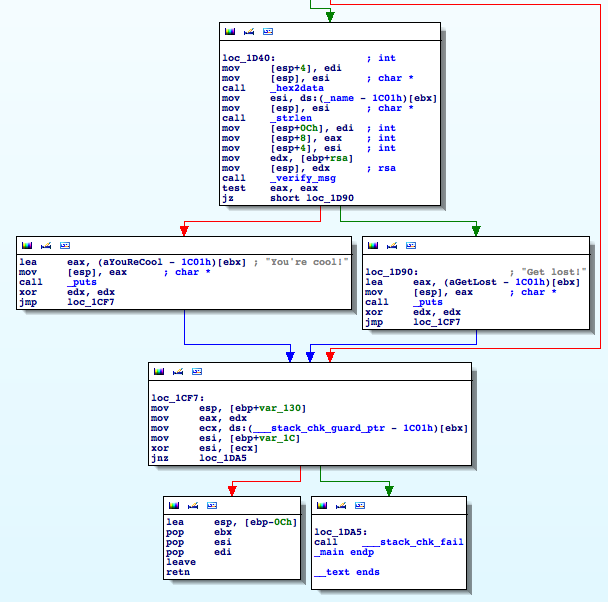
\includegraphics[width=0.85\textwidth]{IDA-pro-flowchart.png}
  \end{center}
  \caption{Flussdiagramm eines Programmsegments im IDA Pro Disassembler}
\end{figure}

Da diese Disassembler oft auch auf Seiten der Virenentwicklers zum Grundwerkzeug gehören, werden in der Praxis oft Verschleierungs- oder sogar Verschlüsselungstechniken eingesetzt, die statische Code-Analyse erschweren oder unmöglich machen. Die meisten Disassembler sind aber gleichzeitig auch Debugger und erlauben die Analyse zur Laufzeit – bei Schadcode meist in einer gesicherten Laborumgebung. Ein \emph{Trace} durch den Programmablauf hinterlässt dann eine Spur des tatsächlich ausgeführten, aktiven Codes.

Das Umgehen von Software-Sicherungen als Kopier- oder Zugangsschutz ist ein anderes Einsatzfeld von Reverse-Engineering-Techniken in einer legalen Grauzone. Die Verwertung  der Ergebnisse solcher Analysen bricht in der Regel geltendes Patent-, Eigentums- und/oder Urheberrecht. Es gibt jedoch auch Enthusiasten, die \emph{Cracking} aus ``sportlichen'' Gründen betreiben und von den facettenreichen Fähigkeiten fasziniert sind die dazu häufig nötig sind. Ein legaler Weg beschreiten sogenannte \emph{Crackmes}\cite{crackme}, kleine Programme die von anderen \emph{Reversern} geschrieben wurden um sich gegenseitig auszuprobieren oder herauszufordern.

Ein weiteres Gebiet in dem Assembler-Code geschrieben und gelesen werden, muss ist das Entwickeln bzw. Analysieren von \emph{Exploits}. So bezeichnet man kurze Programme zum aktiven Ausnutzen von Sicherheitslücken. Meist geht es dabei darum subversiv, eigenen Code in fremde Computersysteme einzuschleusen und sich nicht-autorisierten Zugang zu verschaffen. Assembler taucht hier meist in Form von \emph{Shellcode} auf. Code der so heißt, da er in der Regel zum Starten einer privilegierten, fernsteuerbaren Shell auf dem Fremdsystem eingeschleust wird. Der Shellcode wird in Form einer mit falscher Absicht zusammengesetzten Dateneingabe eingebracht, auf die die entgegennehmende Software fehlerhaft reagiert. Der Shellcode befindet sich dann schon auf dem Stack oder Heap des anfälligen Programms und muss geschickt unter Ausnutzung der Sicherheitslücke angesprungen werden. Gute Assemblerkentnisse sind für den Exploit-Programmierer Voraussetzung. Die Motivationen sind wiederum vielschichtig und reichen von wissenschaftlichem Forschungsgeist über persönlichen Ehrgeiz bis zu kriminelle Absichten.


\section{Fazit}
Aus heutiger Sicht hat sich die Bedeutung und Verwendung vom x86-Assembler stark verändert.
Wurden vor 20 Jahren noch viele Programme hardwarenah programmiert, so ist dies heutzutage nur noch bedingt der Fall.
Die Lesbarkeit und Wartbarkeit können nicht mit denen von aktuellen Hochsprachen wie Java oder Python mithalten.
Dennoch ist ein Grundverständnis von Assembler wichtig, da letztendlich jede Hochsprache in einen Assembler ähnlichen Maschinencode übersetzt wird.

Ein immer mehr an Bedeutung gewinnender Aspekt in der Informatik ist die Analyse von Schadsoftware.
Das Verhalten von Viren und Würmer lassen sich genau mittels \textit{Reverse Engineering} analysieren.
Hier ist das Wissen über die vorherrschende Computerarchitektur unabdingbar.

Abschließend lässt sich sagen, dass ein Grundverständnis von Assembler durchaus wichtig ist.
Es kann als das Latein des Computers verstanden werden.
Weder wird Latein noch von vielen Menschem im alltäglichen Leben gesprochen, noch wird x86-Assembler bei größeren Software-Projekten als \textit{general-purpose Language} eingesetzt.
Dennoch lassen sich gewisse Grundproblematiken nicht durch Hochsprachen wegabstrahieren und so sind hardwarenahe Programmierkentnisse nicht zu unterschätzen.


\begin{frame}{Quellen}
  % You might wish to add the option [pausesections]
\end{frame}


\end{document}

